
\centerline{\textbf{ \LARGE Data Path }}

\begin{questyle}
  \question  Consider the following data path of a simple non-pilelined CPU. The registers A, B, A1, A2, MDR,
             the bus and the ALU are 8-bit wide. SP and MAR are 16-bit registers. The MUX is of
             size 8 × (2:1) and the DEMUX is of size 8 × (1:2). Each memory operation takes 2 CPU
             clock cycles and uses MAR (Memory Address Register) and MDR (Memory Date Register).
             SP can be decremented locally. How many CPU clock cycles are needed to execute the
             "push r" instruction? The CPU instruction \mbox{"push r"}, where = A or B, has
             following specification. (GATE-2001) \\ M[SP]\(\leftarrow\)r \\ SP\(\leftarrow\)(SP – 1)

             \begin{myTableStyle} \begin{tabular}{ |m{14cm}| } \hline
                  \begin{center} 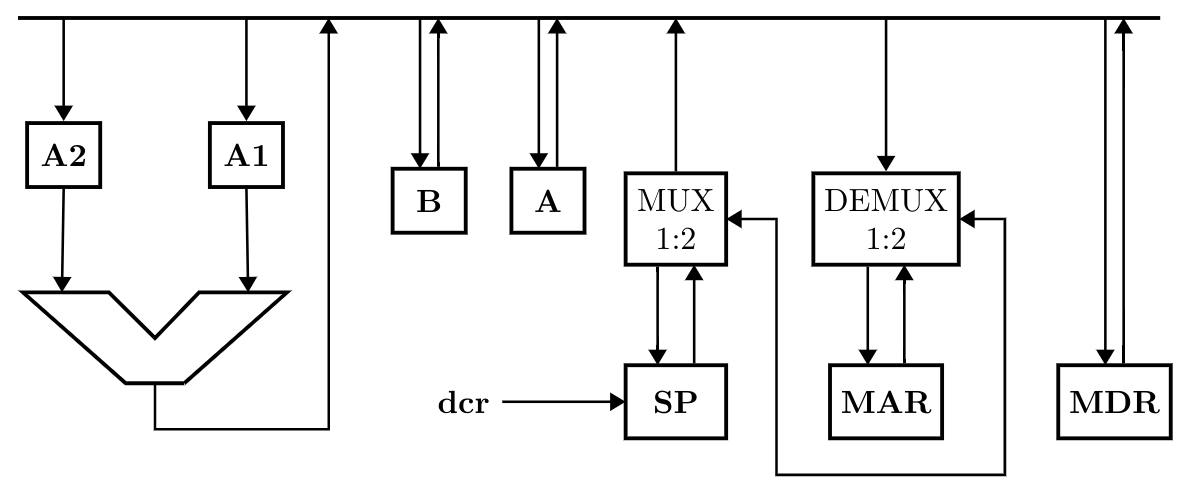
\includegraphics[scale=0.3]{./images/data_path_01.png} \end{center}\\ \hline
            \end{tabular} \end{myTableStyle} \vspace{0.08in}

  \begin{oneparchoices}
    \choice         2
    \choice         3
    \choice         4
    \CorrectChoice  5
  \end{oneparchoices}
  \\ Hint: \qquad CPU has to fill MAR and MDR before memory operation takes place.
  \\ Hint: \qquad 2-cycles \qquad \qquad MAR(2 Byte) \(\leftarrow\) SP(2 Byte) \quad using 8-bit bus
  \\ Hint: \qquad 1-cycles \qquad \qquad MDR(1 Byte) \(\leftarrow\) A(1 Byte) \quad using 8-bit bus
  \\ Hint: \qquad 2-cycles \qquad \qquad Memory Operation
\end{questyle}


\begin{comment}


\begin{questyle}
  \question  zzz  (GATE-zzz)

  \begin{choices}
    \choice         zzz
    \choice         zzz
    \choice         zzz
    \choice         zzz
\CorrectChoice
  \end{choices}
\end{questyle}

\begin{questyle}
  \question  zzz  (GATE-zzz)

  \begin{choices}
    \choice         zzz
    \choice         zzz
    \choice         zzz
    \choice         zzz
\CorrectChoice
  \end{choices}
\end{questyle}

\begin{questyle}
  \question  zzz  (GATE-zzz)

  \begin{choices}
    \choice         zzz
    \choice         zzz
    \choice         zzz
    \choice         zzz
\CorrectChoice
  \end{choices}
\end{questyle}

\end{comment}
